\section{책 페이지 넘기기}

\begin{frame} % No title at first slide
    \sectiontitlenonumber{책 페이지 넘기기}
    \sectionmeta{
        \texttt{simulation, stack}\\
        난이도 -- \textbf{\color{acbronze}Easy}
    }
    \begin{itemize}
        \item 
    \end{itemize}
\end{frame}


\begin{frame}{책 페이지 넘기기}
준식이는 책을 읽으려고 한다. 책은 표지를 포함해 $N$개의 종이로 이루어져 있고, $i$번째 종이에는 앞뒤로 알파벳 $S[i]$가 적혀있다. 준식이는 현재 펼친 페이지에서 왼쪽 페이지나 오른쪽 페이지로 이동할 수 있다.

\begin{center}
  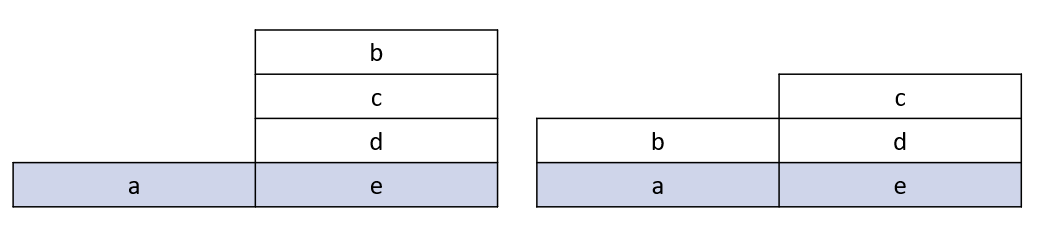
\includegraphics[width=\textwidth]{{images/book-sweep/1.png}} \\
\end{center}

위 그림은 \texttt{abcde}로 이루어진 책의 $1$번째 페이지(\texttt{a})와 $2$번째 페이지(\texttt{b})를 펼쳐 놓은 상태에서 다음 페이지로 넘어간 상황이다. 이제  $2$번째 페이지(\texttt{b})와 $3$번째 페이지(\texttt{c})가 보인다.

준식이는 책을 펼쳐 놓은 상태에서 보이는 왼쪽 페이지나 오른쪽 페이지를 찢어서 떼어낼 수도 있다. 단, 표지는 튼튼하기 때문에 떼어낼 수 없다.

\begin{center}
  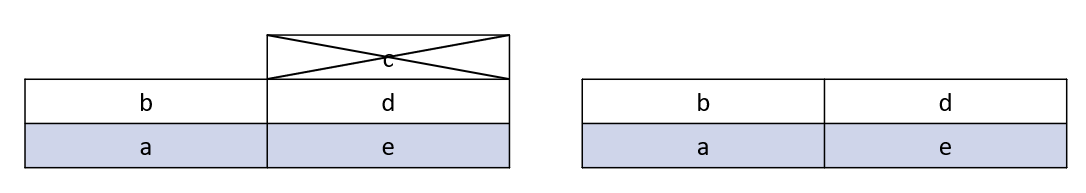
\includegraphics[width=\textwidth]{{images/book-sweep/2.png}} \\
\end{center}

위 그림은 전 그림의 상황에서 오른쪽 페이지(\texttt{c})를 찢어서 떼어낸 상황이다.

책의 각 페이지에 적힌 알파벳과 준식이의 행동이 주어질 때 행동이 모두 끝난 후 보이는 두 페이지를 구해보자.
\end{frame}


\begin{frame}{책 페이지 넘기기 입출력}
첫째 줄에 책의 각 페이지에 적힌 알파벳들이 주어진다. 책의 페이지 개수 $N$은 $2$이상 $100\,000$이하의 양의 정수이다.

\begin{center}
  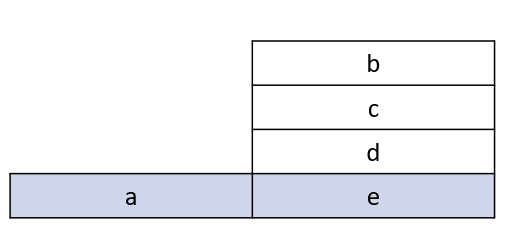
\includegraphics[width=\textwidth]{{images/book-sweep/3.png}} \\
\end{center}

초기 상태에서 보이는 페이지는 $1$번째 페이지(\texttt{a})와 $2$번째 페이지(\texttt{b})이다. 위 그림을 참고한다.

둘째 줄에 준식이의 행동의 개수 $M(1 \leq M \leq 100\,000)$이 주어진다. 

셋째 줄부터 $M$개의 줄에 준식이의 행동이 주어진다. 준식이의 행동은 다음 중 하나이다.

\texttt{prev} 이전 페이지로 넘어간다. 만약 왼쪽에 보이는 페이지가 표지라면 아무 행동도 하지 않는다.

\texttt{next} 다음 페이지로 넘어간다. 만약 오른쪽에 보이는 페이지가 표지라면 아무 행동도 하지 않는다.

\texttt{left} 왼쪽 페이지를 찢어서 떼어낸다. 만약 왼쪽에 보이는 페이지가 표지라면 아무 행동도 하지 않는다.

\texttt{right} 오른쪽 페이지를 찢어서 떼어낸다. 만약 오른쪽에 보이는 페이지가 표지라면 아무 행동도 하지 않는다.

준식이의 행동이 모두 끝난 후에 보이는 두 페이지에 적혀있는 알파벳을 출력한다.
\end{frame}


\begin{frame}[fragile]{책 페이지 넘기기 예제 입출력}
\begin{minted}[linenos,fontsize=\scriptsize,frame=single]{text}
abcde
2
next
right
->b d

abcde
6
next
next
next
right
right
right
->d e

abcde
8
next
next
next
prev
prev
right
right
right
->b e

\end{minted}
\end{frame}


\begin{frame}{책 페이지 넘기기 풀이}
    \begin{itemize}
        \item 
    \end{itemize}
\end{frame}


\begin{frame}[fragile]{책 페이지 넘기기 java 정답}
\begin{minted}[linenos,fontsize=\scriptsize,frame=single]{java}
import java.util.*;
import java.io.*;

public class Java {

    public static void main(String[] args) throws IOException {
        BufferedReader br = new BufferedReader(new InputStreamReader(System.in));
        String s = br.readLine();

        Stack<Character> left = new Stack<>();
        Stack<Character> right = new Stack<>();

        left.push(s.charAt(0));
        for (int i = s.length() - 1; i >= 1; i--) {
            right.push(s.charAt(i));
        }

        int m = Integer.parseInt(br.readLine());
        for (int i = 0; i < m; i++) {
            String cmd = br.readLine();

            if (cmd.equals("prev") && left.size() > 1) {
                right.push(left.pop());
            } else if (cmd.equals("next") && right.size() > 1) {
                left.push(right.pop());
            } else if (cmd.equals("left") && left.size() > 1) {
                left.pop();
            } else if (cmd.equals("right") && right.size() > 1) {
                right.pop();
            }
        }

        System.out.print(left.peek() + " " + right.peek());
    }

}

\end{minted}
\end{frame}


\begin{frame}[fragile]{책 페이지 넘기기 python 정답}
\begin{minted}[linenos,fontsize=\scriptsize,frame=single]{python}
s = input()
left, right = [s[0]], [*s[-1:0:-1]]

m = int(input())
for i in range(m):
    cmd = input()

    if cmd == "prev" and len(left) > 1:
        right.append(left.pop())
    elif cmd == "next" and len(right) > 1:
        left.append(right.pop())
    elif cmd == "left" and len(left) > 1:
        left.pop()
    elif cmd == "right" and len(right) > 1:
        right.pop()

print(left[-1], right[-1])

\end{minted}
\end{frame}
